\documentclass[twoside]{book}

% Packages required by doxygen
\usepackage{fixltx2e}
\usepackage{calc}
\usepackage{doxygen}
\usepackage[export]{adjustbox} % also loads graphicx
\usepackage{graphicx}
\usepackage[utf8]{inputenc}
\usepackage{makeidx}
\usepackage{multicol}
\usepackage{multirow}
\PassOptionsToPackage{warn}{textcomp}
\usepackage{textcomp}
\usepackage[nointegrals]{wasysym}
\usepackage[table]{xcolor}

% NLS support packages
\usepackage[french]{babel}

% Font selection
\usepackage[T1]{fontenc}
\usepackage[scaled=.90]{helvet}
\usepackage{courier}
\usepackage{amssymb}
\usepackage{sectsty}
\renewcommand{\familydefault}{\sfdefault}
\allsectionsfont{%
  \fontseries{bc}\selectfont%
  \color{darkgray}%
}
\renewcommand{\DoxyLabelFont}{%
  \fontseries{bc}\selectfont%
  \color{darkgray}%
}
\newcommand{\+}{\discretionary{\mbox{\scriptsize$\hookleftarrow$}}{}{}}

% Page & text layout
\usepackage{geometry}
\geometry{%
  a4paper,%
  top=2.5cm,%
  bottom=2.5cm,%
  left=2.5cm,%
  right=2.5cm%
}
\tolerance=750
\hfuzz=15pt
\hbadness=750
\setlength{\emergencystretch}{15pt}
\setlength{\parindent}{0cm}
\setlength{\parskip}{3ex plus 2ex minus 2ex}
\makeatletter
\renewcommand{\paragraph}{%
  \@startsection{paragraph}{4}{0ex}{-1.0ex}{1.0ex}{%
    \normalfont\normalsize\bfseries\SS@parafont%
  }%
}
\renewcommand{\subparagraph}{%
  \@startsection{subparagraph}{5}{0ex}{-1.0ex}{1.0ex}{%
    \normalfont\normalsize\bfseries\SS@subparafont%
  }%
}
\makeatother

% Headers & footers
\usepackage{fancyhdr}
\pagestyle{fancyplain}
\fancyhead[LE]{\fancyplain{}{\bfseries\thepage}}
\fancyhead[CE]{\fancyplain{}{}}
\fancyhead[RE]{\fancyplain{}{\bfseries\leftmark}}
\fancyhead[LO]{\fancyplain{}{\bfseries\rightmark}}
\fancyhead[CO]{\fancyplain{}{}}
\fancyhead[RO]{\fancyplain{}{\bfseries\thepage}}
\fancyfoot[LE]{\fancyplain{}{}}
\fancyfoot[CE]{\fancyplain{}{}}
\fancyfoot[RE]{\fancyplain{}{\bfseries\scriptsize Généré par Doxygen }}
\fancyfoot[LO]{\fancyplain{}{\bfseries\scriptsize Généré par Doxygen }}
\fancyfoot[CO]{\fancyplain{}{}}
\fancyfoot[RO]{\fancyplain{}{}}
\renewcommand{\footrulewidth}{0.4pt}
\renewcommand{\chaptermark}[1]{%
  \markboth{#1}{}%
}
\renewcommand{\sectionmark}[1]{%
  \markright{\thesection\ #1}%
}

% Indices & bibliography
\usepackage{natbib}
\usepackage[titles]{tocloft}
\setcounter{tocdepth}{3}
\setcounter{secnumdepth}{5}
\makeindex

% Hyperlinks (required, but should be loaded last)
\usepackage{ifpdf}
\ifpdf
  \usepackage[pdftex,pagebackref=true]{hyperref}
\else
  \usepackage[ps2pdf,pagebackref=true]{hyperref}
\fi
\hypersetup{%
  colorlinks=true,%
  linkcolor=blue,%
  citecolor=blue,%
  unicode%
}

% Custom commands
\newcommand{\clearemptydoublepage}{%
  \newpage{\pagestyle{empty}\cleardoublepage}%
}

\usepackage{caption}
\captionsetup{labelsep=space,justification=centering,font={bf},singlelinecheck=off,skip=4pt,position=top}

%===== C O N T E N T S =====

\begin{document}

% Titlepage & ToC
\hypersetup{pageanchor=false,
             bookmarksnumbered=true,
             pdfencoding=unicode
            }
\pagenumbering{alph}
\begin{titlepage}
\vspace*{7cm}
\begin{center}%
{\Large Indexation texte }\\
\vspace*{1cm}
{\large Généré par Doxygen 1.8.13}\\
\end{center}
\end{titlepage}
\clearemptydoublepage
\pagenumbering{roman}
\tableofcontents
\clearemptydoublepage
\pagenumbering{arabic}
\hypersetup{pageanchor=true}

%--- Begin generated contents ---
\chapter{Index des fichiers}
\section{Liste des fichiers}
Liste de tous les fichiers documentés avec une brève description \+:\begin{DoxyCompactList}
\item\contentsline{section}{\hyperlink{Header_8h}{Header.\+h} \\*Header de toute la partie Texte }{\pageref{Header_8h}}{}
\item\contentsline{section}{\hyperlink{outils_8c}{outils.\+c} \\*Quelques fonctions annexes nécessaire au bon fonctionnement }{\pageref{outils_8c}}{}
\item\contentsline{section}{\hyperlink{xml__cleaner_8c}{xml\+\_\+cleaner.\+c} \\*Fonctions permettant de nettoyer un fichier xml et d\textquotesingle{}obtenir un .xml }{\pageref{xml__cleaner_8c}}{}
\item\contentsline{section}{\hyperlink{xml__index_8c}{xml\+\_\+index.\+c} \\*Fonctions d\textquotesingle{}indexations et de création de piles de descripteurs }{\pageref{xml__index_8c}}{}
\item\contentsline{section}{\hyperlink{xml__tokenizer_8c}{xml\+\_\+tokenizer.\+c} \\*Fonctions de nettoyage de fichiers .clean }{\pageref{xml__tokenizer_8c}}{}
\end{DoxyCompactList}

\chapter{Documentation des fichiers}
\hypertarget{Header_8h}{}\section{Référence du fichier Header.\+h}
\label{Header_8h}\index{Header.\+h@{Header.\+h}}


Header de toute la partie Texte.  


{\ttfamily \#include \char`\"{}pile/pile\+\_\+dynamique.\+h\char`\"{}}\newline
{\ttfamily \#include $<$ctype.\+h$>$}\newline
{\ttfamily \#include $<$dirent.\+h$>$}\newline
{\ttfamily \#include $<$sys/types.\+h$>$}\newline
{\ttfamily \#include $<$sys/stat.\+h$>$}\newline
Graphe des dépendances par inclusion de Header.\+h\+:
\nopagebreak
\begin{figure}[H]
\begin{center}
\leavevmode
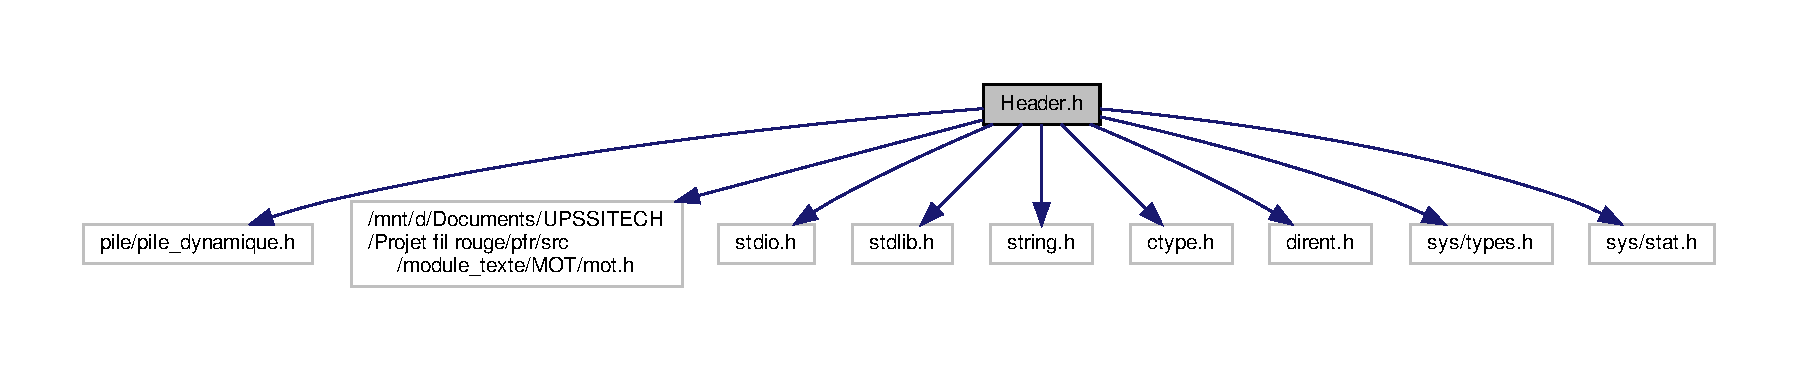
\includegraphics[width=350pt]{Header_8h__incl}
\end{center}
\end{figure}
Ce graphe montre quels fichiers incluent directement ou indirectement ce fichier \+:
\nopagebreak
\begin{figure}[H]
\begin{center}
\leavevmode
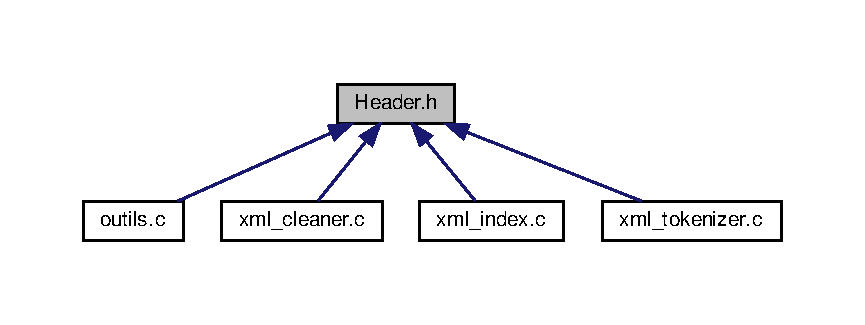
\includegraphics[width=350pt]{Header_8h__dep__incl}
\end{center}
\end{figure}
\subsection*{Macros}
\begin{DoxyCompactItemize}
\item 
\mbox{\Hypertarget{Header_8h_a392fb874e547e582e9c66a08a1f23326}\label{Header_8h_a392fb874e547e582e9c66a08a1f23326}} 
\#define {\bfseries M\+AX}~512
\end{DoxyCompactItemize}
\subsection*{Fonctions}
\begin{DoxyCompactItemize}
\item 
void \hyperlink{Header_8h_ab3ff0edee79903c931ae1cc1be78e1c6}{Descripteur\+\_\+texte\+\_\+fichier} (char $\ast$nom\+\_\+fichier, P\+I\+L\+E\+\_\+descripteur\+\_\+texte $\ast$pile\+\_\+desc)
\begin{DoxyCompactList}\small\item\em Permet d\textquotesingle{}obtenir un descripteur texte à partir du chemin d\textquotesingle{}un fichier xml. \end{DoxyCompactList}\item 
int \hyperlink{Header_8h_a47f1db2fb139f2d254299930debddd1d}{Descripteur\+\_\+texte\+\_\+dossier} (char $\ast$nom\+\_\+dossier, P\+I\+L\+E\+\_\+descripteur\+\_\+texte $\ast$pile\+\_\+desc)
\begin{DoxyCompactList}\small\item\em Permet d\textquotesingle{}obtenir tous les descripteurs texte présents dans un dossier. \end{DoxyCompactList}\item 
void \hyperlink{Header_8h_ae541103221499ab14d680ed40958a049}{xml\+\_\+cleaner} (F\+I\+LE $\ast$src, F\+I\+LE $\ast$dest)
\begin{DoxyCompactList}\small\item\em Permet de passer d\textquotesingle{}un fichier source xml brut à un fichier dest \char`\"{}nettoyé\char`\"{} de ses balises. \end{DoxyCompactList}\item 
void \hyperlink{Header_8h_a25a265268495488b4b060c9a6e394105}{xml\+\_\+filter} (F\+I\+LE $\ast$src, F\+I\+LE $\ast$dest)
\begin{DoxyCompactList}\small\item\em Permet d\textquotesingle{}obtenir un fichier \char`\"{}nettoyé\char`\"{} de ses stopwords ainsi que de sa ponctuation (et des majuscules) \end{DoxyCompactList}\item 
void \hyperlink{Header_8h_a425c9a0a21cf3d96fd4c12f4b0ebb37d}{lecture\+\_\+dossier} (F\+I\+LE $\ast$f, char $\ast$nom\+\_\+dossier)
\begin{DoxyCompactList}\small\item\em Permet de récupérer les noms de chaque fichier (qui ne sont pas des dossiers) \end{DoxyCompactList}\item 
void \hyperlink{Header_8h_a5a1f0bfe6b0d9368768dab1e9bfcda74}{path\+\_\+maker} (char $\ast$chemin, char $\ast$nom\+\_\+dossier, char $\ast$nom\+\_\+fichier)
\begin{DoxyCompactList}\small\item\em Permet de mettre un chemin vers un fichier sous forme de chaine de caracteres. \end{DoxyCompactList}\end{DoxyCompactItemize}


\subsection{Description détaillée}
Header de toute la partie Texte. 

\begin{DoxyAuthor}{Auteur}
Baptiste P\+O\+M\+A\+R\+E\+L\+LE 
\end{DoxyAuthor}
\begin{DoxyVersion}{Version}
0.\+1 
\end{DoxyVersion}
\begin{DoxyDate}{Date}
2020-\/12-\/16
\end{DoxyDate}
\begin{DoxyCopyright}{Copyright}
Copyright (c) 2020 
\end{DoxyCopyright}


\subsection{Documentation des fonctions}
\mbox{\Hypertarget{Header_8h_a47f1db2fb139f2d254299930debddd1d}\label{Header_8h_a47f1db2fb139f2d254299930debddd1d}} 
\index{Header.\+h@{Header.\+h}!Descripteur\+\_\+texte\+\_\+dossier@{Descripteur\+\_\+texte\+\_\+dossier}}
\index{Descripteur\+\_\+texte\+\_\+dossier@{Descripteur\+\_\+texte\+\_\+dossier}!Header.\+h@{Header.\+h}}
\subsubsection{\texorpdfstring{Descripteur\+\_\+texte\+\_\+dossier()}{Descripteur\_texte\_dossier()}}
{\footnotesize\ttfamily int Descripteur\+\_\+texte\+\_\+dossier (\begin{DoxyParamCaption}\item[{char $\ast$}]{nom\+\_\+dossier,  }\item[{P\+I\+L\+E\+\_\+descripteur\+\_\+texte $\ast$}]{pile\+\_\+desc }\end{DoxyParamCaption})}



Permet d\textquotesingle{}obtenir tous les descripteurs texte présents dans un dossier. 


\begin{DoxyParams}[1]{Paramètres}
\mbox{\tt in}  & {\em nom\+\_\+dossier} & Dossier a traiter \\
\hline
\mbox{\tt in,out}  & {\em pile\+\_\+desc} & pile de descripteurs dans laquelle on ajoute les descripteurs créés \\
\hline
\end{DoxyParams}
\begin{DoxyReturn}{Renvoie}
int 1 si ça a marché, 0 sinon 
\end{DoxyReturn}
\mbox{\Hypertarget{Header_8h_ab3ff0edee79903c931ae1cc1be78e1c6}\label{Header_8h_ab3ff0edee79903c931ae1cc1be78e1c6}} 
\index{Header.\+h@{Header.\+h}!Descripteur\+\_\+texte\+\_\+fichier@{Descripteur\+\_\+texte\+\_\+fichier}}
\index{Descripteur\+\_\+texte\+\_\+fichier@{Descripteur\+\_\+texte\+\_\+fichier}!Header.\+h@{Header.\+h}}
\subsubsection{\texorpdfstring{Descripteur\+\_\+texte\+\_\+fichier()}{Descripteur\_texte\_fichier()}}
{\footnotesize\ttfamily void Descripteur\+\_\+texte\+\_\+fichier (\begin{DoxyParamCaption}\item[{char $\ast$}]{nom\+\_\+fichier,  }\item[{P\+I\+L\+E\+\_\+descripteur\+\_\+texte $\ast$}]{pile\+\_\+desc }\end{DoxyParamCaption})}



Permet d\textquotesingle{}obtenir un descripteur texte à partir du chemin d\textquotesingle{}un fichier xml. 


\begin{DoxyParams}[1]{Paramètres}
\mbox{\tt in}  & {\em nom\+\_\+fichier} & nom du fichier texte \\
\hline
\mbox{\tt in,out}  & {\em pile\+\_\+desc} & pile de descripteurs dans laquelle on ajoute le descripteur créé \\
\hline
\end{DoxyParams}
\mbox{\Hypertarget{Header_8h_a425c9a0a21cf3d96fd4c12f4b0ebb37d}\label{Header_8h_a425c9a0a21cf3d96fd4c12f4b0ebb37d}} 
\index{Header.\+h@{Header.\+h}!lecture\+\_\+dossier@{lecture\+\_\+dossier}}
\index{lecture\+\_\+dossier@{lecture\+\_\+dossier}!Header.\+h@{Header.\+h}}
\subsubsection{\texorpdfstring{lecture\+\_\+dossier()}{lecture\_dossier()}}
{\footnotesize\ttfamily void lecture\+\_\+dossier (\begin{DoxyParamCaption}\item[{F\+I\+LE $\ast$}]{f,  }\item[{char $\ast$}]{nom\+\_\+dossier }\end{DoxyParamCaption})}



Permet de récupérer les noms de chaque fichier (qui ne sont pas des dossiers) 


\begin{DoxyParams}[1]{Paramètres}
\mbox{\tt in}  & {\em f} & le descripteur du fichier dans lequel on va enregistrer les noms de fichiers \\
\hline
\mbox{\tt in}  & {\em nom\+\_\+dossier} & le nom du dossier \\
\hline
\end{DoxyParams}
\mbox{\Hypertarget{Header_8h_a5a1f0bfe6b0d9368768dab1e9bfcda74}\label{Header_8h_a5a1f0bfe6b0d9368768dab1e9bfcda74}} 
\index{Header.\+h@{Header.\+h}!path\+\_\+maker@{path\+\_\+maker}}
\index{path\+\_\+maker@{path\+\_\+maker}!Header.\+h@{Header.\+h}}
\subsubsection{\texorpdfstring{path\+\_\+maker()}{path\_maker()}}
{\footnotesize\ttfamily void path\+\_\+maker (\begin{DoxyParamCaption}\item[{char $\ast$}]{chemin,  }\item[{char $\ast$}]{nom\+\_\+dossier,  }\item[{char $\ast$}]{nom\+\_\+fichier }\end{DoxyParamCaption})}



Permet de mettre un chemin vers un fichier sous forme de chaine de caracteres. 


\begin{DoxyParams}[1]{Paramètres}
\mbox{\tt in,out}  & {\em chemin} & \\
\hline
\mbox{\tt in}  & {\em nom\+\_\+dossier} & \\
\hline
\mbox{\tt in}  & {\em nom\+\_\+fichier} & \\
\hline
\end{DoxyParams}
\mbox{\Hypertarget{Header_8h_ae541103221499ab14d680ed40958a049}\label{Header_8h_ae541103221499ab14d680ed40958a049}} 
\index{Header.\+h@{Header.\+h}!xml\+\_\+cleaner@{xml\+\_\+cleaner}}
\index{xml\+\_\+cleaner@{xml\+\_\+cleaner}!Header.\+h@{Header.\+h}}
\subsubsection{\texorpdfstring{xml\+\_\+cleaner()}{xml\_cleaner()}}
{\footnotesize\ttfamily void xml\+\_\+cleaner (\begin{DoxyParamCaption}\item[{F\+I\+LE $\ast$}]{src,  }\item[{F\+I\+LE $\ast$}]{dest }\end{DoxyParamCaption})}



Permet de passer d\textquotesingle{}un fichier source xml brut à un fichier dest \char`\"{}nettoyé\char`\"{} de ses balises. 


\begin{DoxyParams}[1]{Paramètres}
\mbox{\tt in}  & {\em src} & fichier source a traiter \\
\hline
\mbox{\tt in}  & {\em dest} & fichier de sortie nettoyé \\
\hline
\end{DoxyParams}
\mbox{\Hypertarget{Header_8h_a25a265268495488b4b060c9a6e394105}\label{Header_8h_a25a265268495488b4b060c9a6e394105}} 
\index{Header.\+h@{Header.\+h}!xml\+\_\+filter@{xml\+\_\+filter}}
\index{xml\+\_\+filter@{xml\+\_\+filter}!Header.\+h@{Header.\+h}}
\subsubsection{\texorpdfstring{xml\+\_\+filter()}{xml\_filter()}}
{\footnotesize\ttfamily void xml\+\_\+filter (\begin{DoxyParamCaption}\item[{F\+I\+LE $\ast$}]{src,  }\item[{F\+I\+LE $\ast$}]{dest }\end{DoxyParamCaption})}



Permet d\textquotesingle{}obtenir un fichier \char`\"{}nettoyé\char`\"{} de ses stopwords ainsi que de sa ponctuation (et des majuscules) 


\begin{DoxyParams}[1]{Paramètres}
\mbox{\tt in}  & {\em src} & \\
\hline
\mbox{\tt in}  & {\em dest} & \\
\hline
\end{DoxyParams}

\hypertarget{outils_8c}{}\section{Référence du fichier outils.\+c}
\label{outils_8c}\index{outils.\+c@{outils.\+c}}


Quelques fonctions annexes nécessaire au bon fonctionnement.  


{\ttfamily \#include \char`\"{}Header.\+h\char`\"{}}\newline
Graphe des dépendances par inclusion de outils.\+c\+:
\nopagebreak
\begin{figure}[H]
\begin{center}
\leavevmode
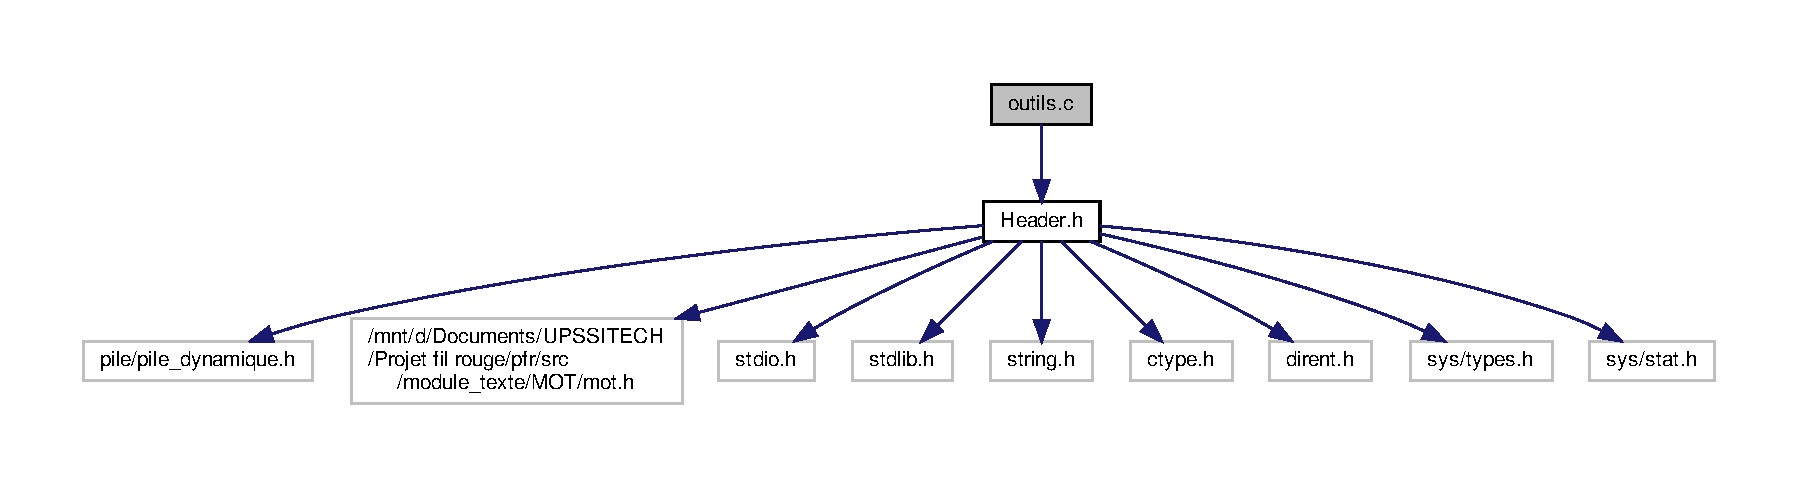
\includegraphics[width=350pt]{outils_8c__incl}
\end{center}
\end{figure}
\subsection*{Fonctions}
\begin{DoxyCompactItemize}
\item 
void \hyperlink{outils_8c_a5a1f0bfe6b0d9368768dab1e9bfcda74}{path\+\_\+maker} (char $\ast$chemin, char $\ast$nom\+\_\+dossier, char $\ast$nom\+\_\+fichier)
\begin{DoxyCompactList}\small\item\em Permet de mettre un chemin vers un fichier sous forme de chaine de caracteres. \end{DoxyCompactList}\item 
void \hyperlink{outils_8c_a425c9a0a21cf3d96fd4c12f4b0ebb37d}{lecture\+\_\+dossier} (F\+I\+LE $\ast$f, char $\ast$nom\+\_\+dossier)
\begin{DoxyCompactList}\small\item\em Permet de récupérer les noms de chaque fichier (qui ne sont pas des dossiers) \end{DoxyCompactList}\end{DoxyCompactItemize}


\subsection{Description détaillée}
Quelques fonctions annexes nécessaire au bon fonctionnement. 

\begin{DoxyAuthor}{Auteur}
Baptiste P\+O\+M\+A\+R\+E\+L\+LE 
\end{DoxyAuthor}
\begin{DoxyVersion}{Version}
0.\+1 
\end{DoxyVersion}
\begin{DoxyDate}{Date}
2020-\/12-\/16
\end{DoxyDate}
\begin{DoxyCopyright}{Copyright}
Copyright (c) 2020 
\end{DoxyCopyright}


\subsection{Documentation des fonctions}
\mbox{\Hypertarget{outils_8c_a425c9a0a21cf3d96fd4c12f4b0ebb37d}\label{outils_8c_a425c9a0a21cf3d96fd4c12f4b0ebb37d}} 
\index{outils.\+c@{outils.\+c}!lecture\+\_\+dossier@{lecture\+\_\+dossier}}
\index{lecture\+\_\+dossier@{lecture\+\_\+dossier}!outils.\+c@{outils.\+c}}
\subsubsection{\texorpdfstring{lecture\+\_\+dossier()}{lecture\_dossier()}}
{\footnotesize\ttfamily void lecture\+\_\+dossier (\begin{DoxyParamCaption}\item[{F\+I\+LE $\ast$}]{f,  }\item[{char $\ast$}]{nom\+\_\+dossier }\end{DoxyParamCaption})}



Permet de récupérer les noms de chaque fichier (qui ne sont pas des dossiers) 


\begin{DoxyParams}[1]{Paramètres}
\mbox{\tt in}  & {\em f} & le descripteur du fichier dans lequel on va enregistrer les noms de fichiers \\
\hline
\mbox{\tt in}  & {\em nom\+\_\+dossier} & le nom du dossier \\
\hline
\end{DoxyParams}
\mbox{\Hypertarget{outils_8c_a5a1f0bfe6b0d9368768dab1e9bfcda74}\label{outils_8c_a5a1f0bfe6b0d9368768dab1e9bfcda74}} 
\index{outils.\+c@{outils.\+c}!path\+\_\+maker@{path\+\_\+maker}}
\index{path\+\_\+maker@{path\+\_\+maker}!outils.\+c@{outils.\+c}}
\subsubsection{\texorpdfstring{path\+\_\+maker()}{path\_maker()}}
{\footnotesize\ttfamily void path\+\_\+maker (\begin{DoxyParamCaption}\item[{char $\ast$}]{chemin,  }\item[{char $\ast$}]{nom\+\_\+dossier,  }\item[{char $\ast$}]{nom\+\_\+fichier }\end{DoxyParamCaption})}



Permet de mettre un chemin vers un fichier sous forme de chaine de caracteres. 


\begin{DoxyParams}[1]{Paramètres}
\mbox{\tt in,out}  & {\em chemin} & \\
\hline
\mbox{\tt in}  & {\em nom\+\_\+dossier} & \\
\hline
\mbox{\tt in}  & {\em nom\+\_\+fichier} & \\
\hline
\end{DoxyParams}

\hypertarget{xml__cleaner_8c}{}\section{Référence du fichier xml\+\_\+cleaner.\+c}
\label{xml__cleaner_8c}\index{xml\+\_\+cleaner.\+c@{xml\+\_\+cleaner.\+c}}


Fonctions permettant de nettoyer un fichier xml et d\textquotesingle{}obtenir un .xml.  


{\ttfamily \#include \char`\"{}Header.\+h\char`\"{}}\newline
Graphe des dépendances par inclusion de xml\+\_\+cleaner.\+c\+:
\nopagebreak
\begin{figure}[H]
\begin{center}
\leavevmode
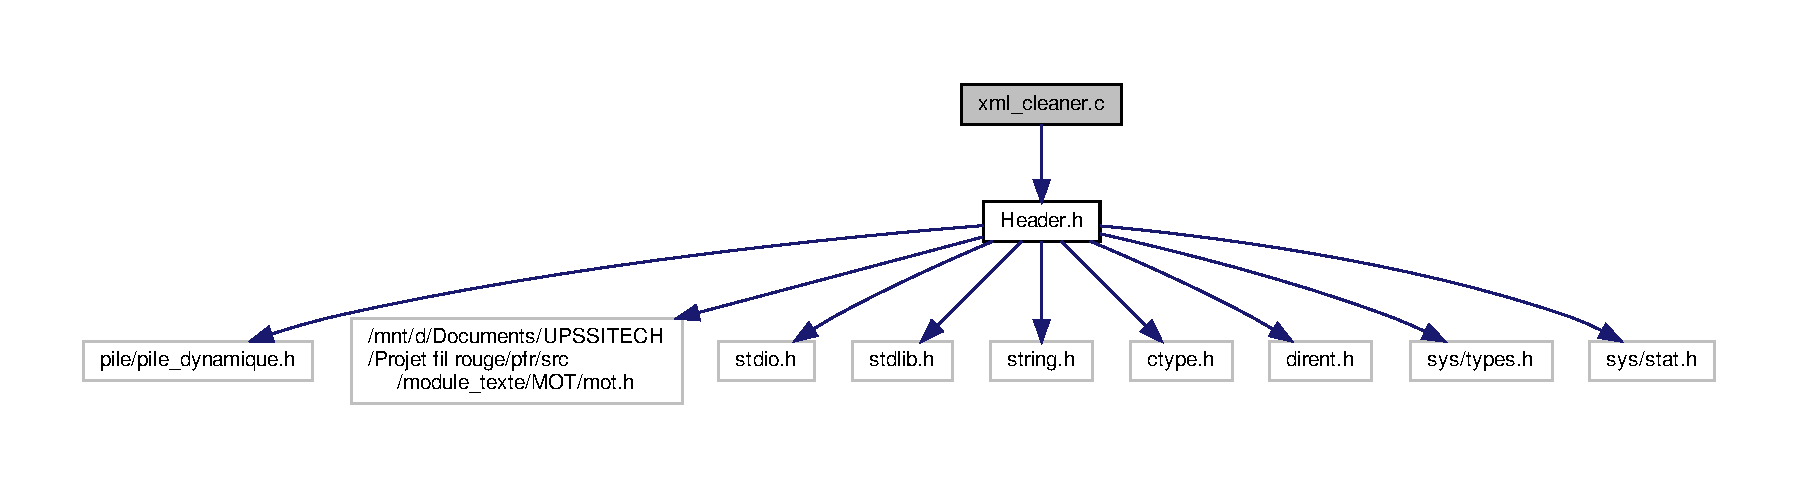
\includegraphics[width=350pt]{xml__cleaner_8c__incl}
\end{center}
\end{figure}
\subsection*{Fonctions}
\begin{DoxyCompactItemize}
\item 
void \hyperlink{xml__cleaner_8c_aff4747721c1e29bc81b8a76cfe8b708d}{add\+\_\+char} (char $\ast$buffer, char c, int $\ast$cpt)
\begin{DoxyCompactList}\small\item\em Permet d\textquotesingle{}ajouter un caractère à une chaine. \end{DoxyCompactList}\item 
int \hyperlink{xml__cleaner_8c_a9a8fd3b9ef561f383766bffef7dd2a1d}{est\+Ponctuation} (char c)
\begin{DoxyCompactList}\small\item\em Permet de déterminer si le caractère donné en paramètre est une ponctuation. \end{DoxyCompactList}\item 
void \hyperlink{xml__cleaner_8c_ae541103221499ab14d680ed40958a049}{xml\+\_\+cleaner} (F\+I\+LE $\ast$src, F\+I\+LE $\ast$dest)
\begin{DoxyCompactList}\small\item\em Permet de passer d\textquotesingle{}un fichier source xml brut à un fichier dest \char`\"{}nettoyé\char`\"{} de ses balises. \end{DoxyCompactList}\end{DoxyCompactItemize}


\subsection{Description détaillée}
Fonctions permettant de nettoyer un fichier xml et d\textquotesingle{}obtenir un .xml. 

\begin{DoxyAuthor}{Auteur}
Baptiste P\+O\+M\+A\+R\+E\+L\+LE 
\end{DoxyAuthor}
\begin{DoxyVersion}{Version}
0.\+1 
\end{DoxyVersion}
\begin{DoxyDate}{Date}
2020-\/12-\/16
\end{DoxyDate}
\begin{DoxyCopyright}{Copyright}
Copyright (c) 2020 
\end{DoxyCopyright}


\subsection{Documentation des fonctions}
\mbox{\Hypertarget{xml__cleaner_8c_aff4747721c1e29bc81b8a76cfe8b708d}\label{xml__cleaner_8c_aff4747721c1e29bc81b8a76cfe8b708d}} 
\index{xml\+\_\+cleaner.\+c@{xml\+\_\+cleaner.\+c}!add\+\_\+char@{add\+\_\+char}}
\index{add\+\_\+char@{add\+\_\+char}!xml\+\_\+cleaner.\+c@{xml\+\_\+cleaner.\+c}}
\subsubsection{\texorpdfstring{add\+\_\+char()}{add\_char()}}
{\footnotesize\ttfamily void add\+\_\+char (\begin{DoxyParamCaption}\item[{char $\ast$}]{buffer,  }\item[{char}]{c,  }\item[{int $\ast$}]{cpt }\end{DoxyParamCaption})}



Permet d\textquotesingle{}ajouter un caractère à une chaine. 


\begin{DoxyParams}[1]{Paramètres}
\mbox{\tt out}  & {\em buffer} & chaine de retour \\
\hline
\mbox{\tt in}  & {\em c} & \\
\hline
\mbox{\tt in}  & {\em cpt} & \\
\hline
\end{DoxyParams}
\mbox{\Hypertarget{xml__cleaner_8c_a9a8fd3b9ef561f383766bffef7dd2a1d}\label{xml__cleaner_8c_a9a8fd3b9ef561f383766bffef7dd2a1d}} 
\index{xml\+\_\+cleaner.\+c@{xml\+\_\+cleaner.\+c}!est\+Ponctuation@{est\+Ponctuation}}
\index{est\+Ponctuation@{est\+Ponctuation}!xml\+\_\+cleaner.\+c@{xml\+\_\+cleaner.\+c}}
\subsubsection{\texorpdfstring{est\+Ponctuation()}{estPonctuation()}}
{\footnotesize\ttfamily int est\+Ponctuation (\begin{DoxyParamCaption}\item[{char}]{c }\end{DoxyParamCaption})}



Permet de déterminer si le caractère donné en paramètre est une ponctuation. 


\begin{DoxyParams}[1]{Paramètres}
\mbox{\tt in}  & {\em c} & \\
\hline
\end{DoxyParams}
\begin{DoxyReturn}{Renvoie}
int 
\end{DoxyReturn}
\mbox{\Hypertarget{xml__cleaner_8c_ae541103221499ab14d680ed40958a049}\label{xml__cleaner_8c_ae541103221499ab14d680ed40958a049}} 
\index{xml\+\_\+cleaner.\+c@{xml\+\_\+cleaner.\+c}!xml\+\_\+cleaner@{xml\+\_\+cleaner}}
\index{xml\+\_\+cleaner@{xml\+\_\+cleaner}!xml\+\_\+cleaner.\+c@{xml\+\_\+cleaner.\+c}}
\subsubsection{\texorpdfstring{xml\+\_\+cleaner()}{xml\_cleaner()}}
{\footnotesize\ttfamily void xml\+\_\+cleaner (\begin{DoxyParamCaption}\item[{F\+I\+LE $\ast$}]{src,  }\item[{F\+I\+LE $\ast$}]{dest }\end{DoxyParamCaption})}



Permet de passer d\textquotesingle{}un fichier source xml brut à un fichier dest \char`\"{}nettoyé\char`\"{} de ses balises. 


\begin{DoxyParams}[1]{Paramètres}
\mbox{\tt in}  & {\em src} & fichier source a traiter \\
\hline
\mbox{\tt in}  & {\em dest} & fichier de sortie nettoyé \\
\hline
\end{DoxyParams}

\hypertarget{xml__index_8c}{}\section{Référence du fichier xml\+\_\+index.\+c}
\label{xml__index_8c}\index{xml\+\_\+index.\+c@{xml\+\_\+index.\+c}}


Fonctions d\textquotesingle{}indexations et de création de piles de descripteurs.  


{\ttfamily \#include \char`\"{}Header.\+h\char`\"{}}\newline
Graphe des dépendances par inclusion de xml\+\_\+index.\+c\+:
\nopagebreak
\begin{figure}[H]
\begin{center}
\leavevmode
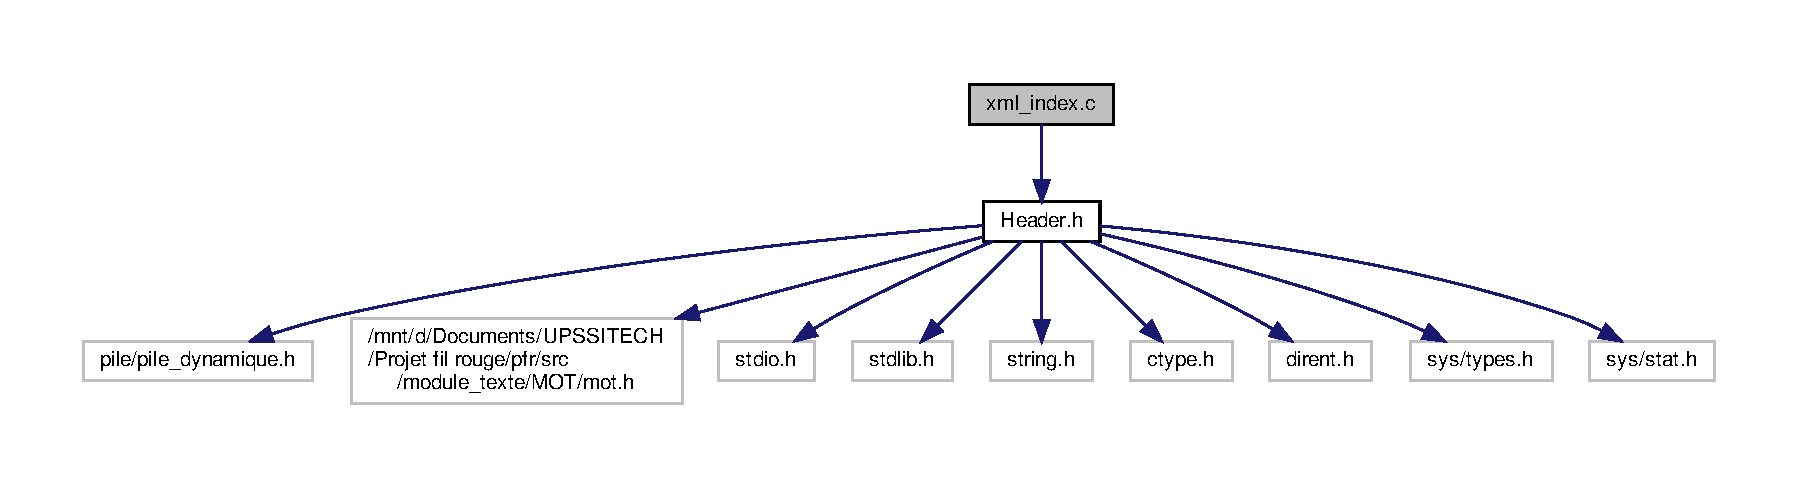
\includegraphics[width=350pt]{xml__index_8c__incl}
\end{center}
\end{figure}
\subsection*{Fonctions}
\begin{DoxyCompactItemize}
\item 
void \hyperlink{xml__index_8c_acffc1df009d3eb1aa80c318c0a585dc2}{descripteur\+\_\+de\+\_\+texte} (F\+I\+LE $\ast$src, P\+I\+LE $\ast$p)
\begin{DoxyCompactList}\small\item\em Permet d\textquotesingle{}obtenir une pile contenant les mots qui apparaissent ainsi que leurs occurences dans le texte. \end{DoxyCompactList}\item 
void \hyperlink{xml__index_8c_a2a272e4e98b1c930fcceff178f60bdd8}{fabrique\+\_\+a\+\_\+descripteur} (char $\ast$path\+\_\+to\+\_\+xml, P\+I\+L\+E\+\_\+descripteur\+\_\+texte $\ast$pile\+\_\+desc)
\begin{DoxyCompactList}\small\item\em Permet de concevoir un descripteur et à l\textquotesingle{}empiler. \end{DoxyCompactList}\item 
int \hyperlink{xml__index_8c_a47f1db2fb139f2d254299930debddd1d}{Descripteur\+\_\+texte\+\_\+dossier} (char $\ast$nom\+\_\+dossier, P\+I\+L\+E\+\_\+descripteur\+\_\+texte $\ast$pile\+\_\+desc)
\begin{DoxyCompactList}\small\item\em Permet d\textquotesingle{}obtenir tous les descripteurs texte présents dans un dossier. \end{DoxyCompactList}\item 
void \hyperlink{xml__index_8c_ab3ff0edee79903c931ae1cc1be78e1c6}{Descripteur\+\_\+texte\+\_\+fichier} (char $\ast$nom\+\_\+fichier, P\+I\+L\+E\+\_\+descripteur\+\_\+texte $\ast$pile\+\_\+desc)
\begin{DoxyCompactList}\small\item\em Permet d\textquotesingle{}obtenir un descripteur texte à partir du chemin d\textquotesingle{}un fichier xml. \end{DoxyCompactList}\item 
\mbox{\Hypertarget{xml__index_8c_a840291bc02cba5474a4cb46a9b9566fe}\label{xml__index_8c_a840291bc02cba5474a4cb46a9b9566fe}} 
int {\bfseries main} (void)
\end{DoxyCompactItemize}


\subsection{Description détaillée}
Fonctions d\textquotesingle{}indexations et de création de piles de descripteurs. 

\begin{DoxyAuthor}{Auteur}
Baptiste P\+O\+M\+A\+R\+E\+L\+LE 
\end{DoxyAuthor}
\begin{DoxyVersion}{Version}
0.\+1 
\end{DoxyVersion}
\begin{DoxyDate}{Date}
2020-\/12-\/16
\end{DoxyDate}
\begin{DoxyCopyright}{Copyright}
Copyright (c) 2020 
\end{DoxyCopyright}


\subsection{Documentation des fonctions}
\mbox{\Hypertarget{xml__index_8c_acffc1df009d3eb1aa80c318c0a585dc2}\label{xml__index_8c_acffc1df009d3eb1aa80c318c0a585dc2}} 
\index{xml\+\_\+index.\+c@{xml\+\_\+index.\+c}!descripteur\+\_\+de\+\_\+texte@{descripteur\+\_\+de\+\_\+texte}}
\index{descripteur\+\_\+de\+\_\+texte@{descripteur\+\_\+de\+\_\+texte}!xml\+\_\+index.\+c@{xml\+\_\+index.\+c}}
\subsubsection{\texorpdfstring{descripteur\+\_\+de\+\_\+texte()}{descripteur\_de\_texte()}}
{\footnotesize\ttfamily void descripteur\+\_\+de\+\_\+texte (\begin{DoxyParamCaption}\item[{F\+I\+LE $\ast$}]{src,  }\item[{P\+I\+LE $\ast$}]{p }\end{DoxyParamCaption})}



Permet d\textquotesingle{}obtenir une pile contenant les mots qui apparaissent ainsi que leurs occurences dans le texte. 


\begin{DoxyParams}[1]{Paramètres}
\mbox{\tt in}  & {\em src} & Descripteur du fichier texte \\
\hline
\mbox{\tt in,out}  & {\em p} & La pile à remplir \\
\hline
\end{DoxyParams}
\mbox{\Hypertarget{xml__index_8c_a47f1db2fb139f2d254299930debddd1d}\label{xml__index_8c_a47f1db2fb139f2d254299930debddd1d}} 
\index{xml\+\_\+index.\+c@{xml\+\_\+index.\+c}!Descripteur\+\_\+texte\+\_\+dossier@{Descripteur\+\_\+texte\+\_\+dossier}}
\index{Descripteur\+\_\+texte\+\_\+dossier@{Descripteur\+\_\+texte\+\_\+dossier}!xml\+\_\+index.\+c@{xml\+\_\+index.\+c}}
\subsubsection{\texorpdfstring{Descripteur\+\_\+texte\+\_\+dossier()}{Descripteur\_texte\_dossier()}}
{\footnotesize\ttfamily int Descripteur\+\_\+texte\+\_\+dossier (\begin{DoxyParamCaption}\item[{char $\ast$}]{nom\+\_\+dossier,  }\item[{P\+I\+L\+E\+\_\+descripteur\+\_\+texte $\ast$}]{pile\+\_\+desc }\end{DoxyParamCaption})}



Permet d\textquotesingle{}obtenir tous les descripteurs texte présents dans un dossier. 


\begin{DoxyParams}[1]{Paramètres}
\mbox{\tt in}  & {\em nom\+\_\+dossier} & Dossier a traiter \\
\hline
\mbox{\tt in,out}  & {\em pile\+\_\+desc} & pile de descripteurs dans laquelle on ajoute les descripteurs créés \\
\hline
\end{DoxyParams}
\begin{DoxyReturn}{Renvoie}
int 1 si ça a marché, 0 sinon 
\end{DoxyReturn}
\mbox{\Hypertarget{xml__index_8c_ab3ff0edee79903c931ae1cc1be78e1c6}\label{xml__index_8c_ab3ff0edee79903c931ae1cc1be78e1c6}} 
\index{xml\+\_\+index.\+c@{xml\+\_\+index.\+c}!Descripteur\+\_\+texte\+\_\+fichier@{Descripteur\+\_\+texte\+\_\+fichier}}
\index{Descripteur\+\_\+texte\+\_\+fichier@{Descripteur\+\_\+texte\+\_\+fichier}!xml\+\_\+index.\+c@{xml\+\_\+index.\+c}}
\subsubsection{\texorpdfstring{Descripteur\+\_\+texte\+\_\+fichier()}{Descripteur\_texte\_fichier()}}
{\footnotesize\ttfamily void Descripteur\+\_\+texte\+\_\+fichier (\begin{DoxyParamCaption}\item[{char $\ast$}]{nom\+\_\+fichier,  }\item[{P\+I\+L\+E\+\_\+descripteur\+\_\+texte $\ast$}]{pile\+\_\+desc }\end{DoxyParamCaption})}



Permet d\textquotesingle{}obtenir un descripteur texte à partir du chemin d\textquotesingle{}un fichier xml. 


\begin{DoxyParams}[1]{Paramètres}
\mbox{\tt in}  & {\em nom\+\_\+fichier} & nom du fichier texte \\
\hline
\mbox{\tt in,out}  & {\em pile\+\_\+desc} & pile de descripteurs dans laquelle on ajoute le descripteur créé \\
\hline
\end{DoxyParams}
\mbox{\Hypertarget{xml__index_8c_a2a272e4e98b1c930fcceff178f60bdd8}\label{xml__index_8c_a2a272e4e98b1c930fcceff178f60bdd8}} 
\index{xml\+\_\+index.\+c@{xml\+\_\+index.\+c}!fabrique\+\_\+a\+\_\+descripteur@{fabrique\+\_\+a\+\_\+descripteur}}
\index{fabrique\+\_\+a\+\_\+descripteur@{fabrique\+\_\+a\+\_\+descripteur}!xml\+\_\+index.\+c@{xml\+\_\+index.\+c}}
\subsubsection{\texorpdfstring{fabrique\+\_\+a\+\_\+descripteur()}{fabrique\_a\_descripteur()}}
{\footnotesize\ttfamily void fabrique\+\_\+a\+\_\+descripteur (\begin{DoxyParamCaption}\item[{char $\ast$}]{path\+\_\+to\+\_\+xml,  }\item[{P\+I\+L\+E\+\_\+descripteur\+\_\+texte $\ast$}]{pile\+\_\+desc }\end{DoxyParamCaption})}



Permet de concevoir un descripteur et à l\textquotesingle{}empiler. 


\begin{DoxyParams}[1]{Paramètres}
\mbox{\tt in}  & {\em path\+\_\+to\+\_\+xml} & chemin vers un fichier xml \\
\hline
\mbox{\tt in,out}  & {\em pile\+\_\+desc} & Pile de descripteurs \\
\hline
\end{DoxyParams}

\hypertarget{xml__tokenizer_8c}{}\section{Référence du fichier xml\+\_\+tokenizer.\+c}
\label{xml__tokenizer_8c}\index{xml\+\_\+tokenizer.\+c@{xml\+\_\+tokenizer.\+c}}


Fonctions de nettoyage de fichiers .clean.  


{\ttfamily \#include \char`\"{}Header.\+h\char`\"{}}\newline
Graphe des dépendances par inclusion de xml\+\_\+tokenizer.\+c\+:
\nopagebreak
\begin{figure}[H]
\begin{center}
\leavevmode
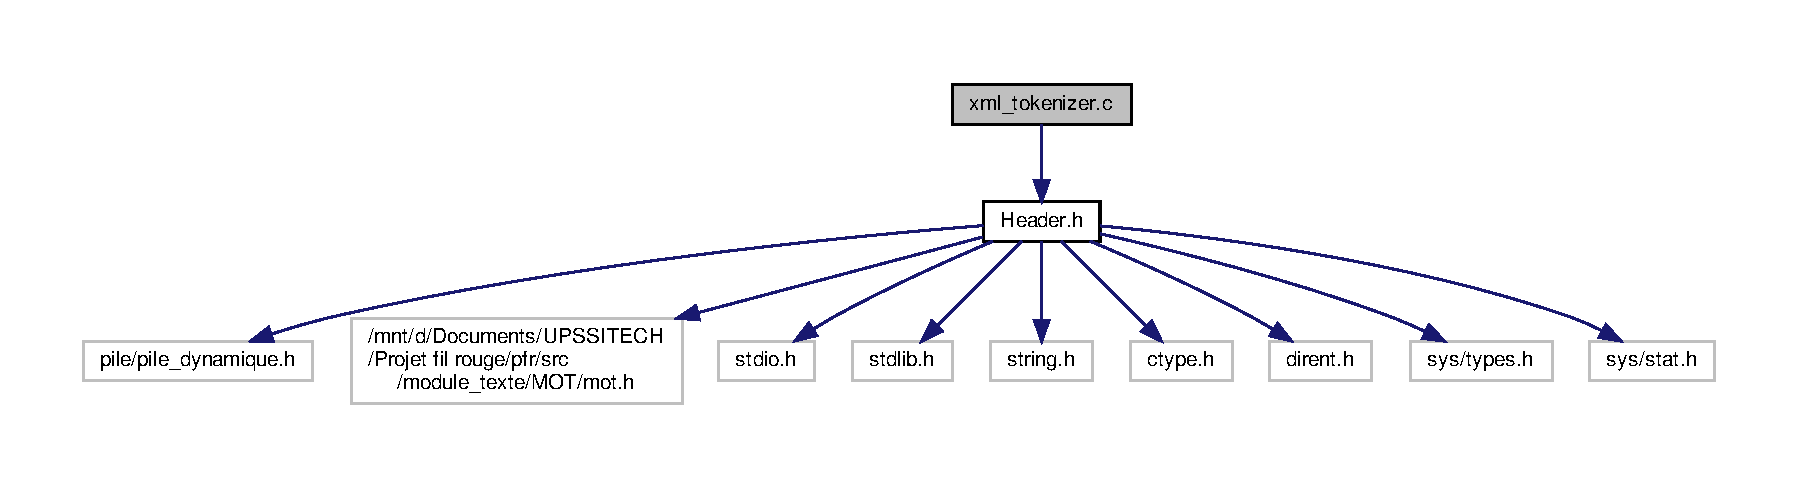
\includegraphics[width=350pt]{xml__tokenizer_8c__incl}
\end{center}
\end{figure}
\subsection*{Fonctions}
\begin{DoxyCompactItemize}
\item 
P\+I\+LE \hyperlink{xml__tokenizer_8c_a04d0c831682d653fc5f8e54461d0129d}{pile\+\_\+stopwords} ()
\begin{DoxyCompactList}\small\item\em Permet de créer une pile contenant tous les stopwords. \end{DoxyCompactList}\item 
void \hyperlink{xml__tokenizer_8c_a25a265268495488b4b060c9a6e394105}{xml\+\_\+filter} (F\+I\+LE $\ast$src, F\+I\+LE $\ast$dest)
\begin{DoxyCompactList}\small\item\em Permet d\textquotesingle{}obtenir un fichier \char`\"{}nettoyé\char`\"{} de ses stopwords ainsi que de sa ponctuation (et des majuscules) \end{DoxyCompactList}\end{DoxyCompactItemize}


\subsection{Description détaillée}
Fonctions de nettoyage de fichiers .clean. 

\begin{DoxyAuthor}{Auteur}
Baptiste P\+O\+M\+A\+R\+E\+L\+LE 
\end{DoxyAuthor}
\begin{DoxyVersion}{Version}
0.\+1 
\end{DoxyVersion}
\begin{DoxyDate}{Date}
2020-\/12-\/16
\end{DoxyDate}
\begin{DoxyCopyright}{Copyright}
Copyright (c) 2020 
\end{DoxyCopyright}


\subsection{Documentation des fonctions}
\mbox{\Hypertarget{xml__tokenizer_8c_a04d0c831682d653fc5f8e54461d0129d}\label{xml__tokenizer_8c_a04d0c831682d653fc5f8e54461d0129d}} 
\index{xml\+\_\+tokenizer.\+c@{xml\+\_\+tokenizer.\+c}!pile\+\_\+stopwords@{pile\+\_\+stopwords}}
\index{pile\+\_\+stopwords@{pile\+\_\+stopwords}!xml\+\_\+tokenizer.\+c@{xml\+\_\+tokenizer.\+c}}
\subsubsection{\texorpdfstring{pile\+\_\+stopwords()}{pile\_stopwords()}}
{\footnotesize\ttfamily P\+I\+LE pile\+\_\+stopwords (\begin{DoxyParamCaption}{ }\end{DoxyParamCaption})}



Permet de créer une pile contenant tous les stopwords. 

\begin{DoxyReturn}{Renvoie}
P\+I\+LE pile de stopwords 
\end{DoxyReturn}
\mbox{\Hypertarget{xml__tokenizer_8c_a25a265268495488b4b060c9a6e394105}\label{xml__tokenizer_8c_a25a265268495488b4b060c9a6e394105}} 
\index{xml\+\_\+tokenizer.\+c@{xml\+\_\+tokenizer.\+c}!xml\+\_\+filter@{xml\+\_\+filter}}
\index{xml\+\_\+filter@{xml\+\_\+filter}!xml\+\_\+tokenizer.\+c@{xml\+\_\+tokenizer.\+c}}
\subsubsection{\texorpdfstring{xml\+\_\+filter()}{xml\_filter()}}
{\footnotesize\ttfamily void xml\+\_\+filter (\begin{DoxyParamCaption}\item[{F\+I\+LE $\ast$}]{src,  }\item[{F\+I\+LE $\ast$}]{dest }\end{DoxyParamCaption})}



Permet d\textquotesingle{}obtenir un fichier \char`\"{}nettoyé\char`\"{} de ses stopwords ainsi que de sa ponctuation (et des majuscules) 


\begin{DoxyParams}[1]{Paramètres}
\mbox{\tt in}  & {\em src} & \\
\hline
\mbox{\tt in}  & {\em dest} & \\
\hline
\end{DoxyParams}

%--- End generated contents ---

% Index
\backmatter
\newpage
\phantomsection
\clearemptydoublepage
\addcontentsline{toc}{chapter}{Index}
\printindex

\end{document}
